\chapter{Interval filament graphs}

\begin{defn}
	Given a half-plane $\pi$ with a border-line $l$, an \textbf{interval filament} in $\pi$ is a simple curve with
	endpoints on $l$, its interior lying in $\pi$ and within the stripe determined by lines perpendicular to $l$ and
	passing through the endpoints of the curve. The class of \textbf{interval filament graphs} is $\text{IFA} = \mathcal{IG}\{\text{interval filaments in a half-plane}\}$.
\end{defn}

\begin{figure}[!ht]\centering
	\begin{tikzpicture}
		\draw[color = gray] (2,0) -- (10,0);
		\node at (3,.3) {$l$};
		\draw[color=black, thick] (5,.01) edge (10,.01);
		\draw[dotted] (5,0) edge (5, 5);
		\draw[dotted] (10,0) edge (10,5);
		
		\draw[color=Red, thick] (5, .01) .. controls (10,5) and (4,3) .. (7, 4);
		\draw[color=Red, thick] (7, 4) .. controls (11,1) and (1,1) .. (10, .01);
		
		\fill[color=Red] (7,4) circle[radius=.35pt];
	\end{tikzpicture}
	\caption{An illustration to the definition. The name “interval-filament” comes from the fact that the curve “lives above” the interval that is determined by the endpoints of the filament on the boundary line $l$.}
\end{figure}

\begin{comm}
	If the base intervals of two interval-filaments overlap (i.e., they are not disjoint, but none of them is a subinterval of the other one), the filaments necessarily cross each other and the corresponding vertices in the intersection graph are adjacent (cf. the blue and red filaments in Fig. \ref{filaments}). On the other hand, if one of the base intervals is included in the other one, their filaments may or may not be disjoint (cf. the blue and yellow filaments for the disjoint case, and the red and green filaments for the non-disjoint one, both in Fig. \ref{filaments}).
\end{comm}

\begin{figure}[!ht]\centering
	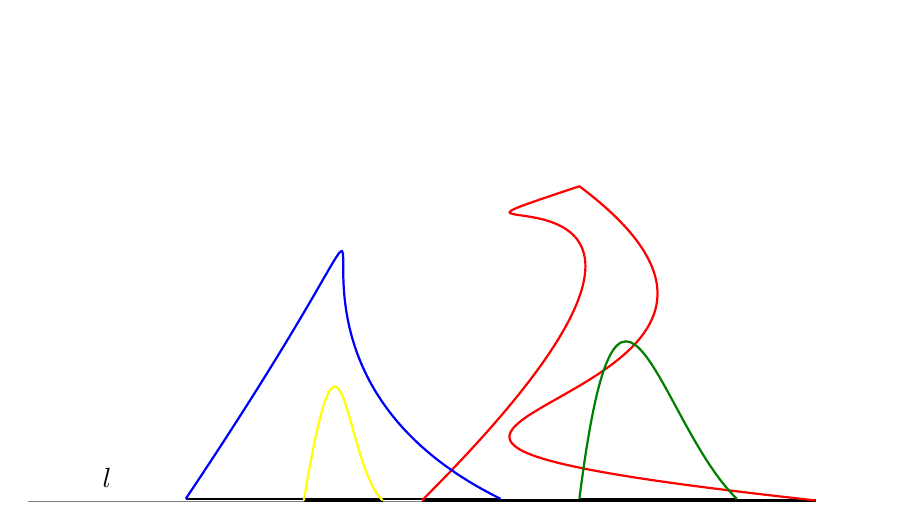
\begin{tikzpicture}
		\draw[color = gray] (0,0) -- (10,0);
		\node at (1,.3) {$l$};
		
		\draw[color=black, thick] (5,.01) edge (10,.01);
		\draw[color=black, thick] (7,.03) edge (9,.03);
		\draw[color=black, thick] (2,.03) edge (6,.03);
		\draw[color=black, thick] (3.5,.01) edge (4.5,.01);
		
		\draw[color=Red, thick] (5, .01) .. controls (10,5) and (4,3) .. (7, 4);
		\draw[color=Red, thick] (7, 4) .. controls (11,1) and (1,1) .. (10, .01);
		\fill[color=Red] (7,4) circle[radius=.35pt];
		
		\draw[color=Yellow, thick] (3.5, .01) .. controls (4,3) and (4,.5) .. (4.5, .01);
		\draw[color=Blue, thick] (2, .03) .. controls (6,6) and (2,2) .. (6, .03);
		\draw[color=Green, thick] (7, .03) .. controls (7.5,4) and (8,1) .. (9, .03);
	\end{tikzpicture}
	\caption{An illustration to the possible relative positions of interval-filaments.}
	\label{filaments}
\end{figure}

\begin{observ}
	$\text{IFA}$ contains $\text{INT}$, $\text{CHOR}$, $\text{FUN}$, $\text{CIR}$, $\text{CA}$, and $\text{PC}$.
\end{observ}

\begin{defn}[class $\mathcal{A}$-mixed]
	Let $\mathcal{A}$ be a graph class. A graph $G = (V, E)$ belongs to the class $\mathcal{A}$-mixed if its edge set allows a partition $E = E_1 \cup E_2$ and a transitive orientation $\overrightarrow{E_2}$ of $E_2$ such that for any three vertices $u, v, w \in V(G)$, $uv \in \overrightarrow{E_2}$ and $vw \in E_1$ imply $uw \in E_1$.
\end{defn}

\begin{thm}
	co-IFA = (co-INT)-mixed.
\end{thm}

\begin{proof}
	"$\subseteq$": Let $G = (V, E) \in \text{IFA}$ and let $\{f_u : u \in V\}$ be an interval-filament representation of $G$, with $f_u$ being a filament with its base interval $I_u$ lying on a common line $l$. Then its complement $-G$ is in co-IFA, and our goal is to show that $-G \in$ (co-INT)-mixed. Define
	
	$$
	E_1 = \{uv : I_u \cap I_v = \emptyset\}
	$$
	
	and
	
	$$
	E_2 = \{uv : ((I_u \subseteq I_v ) \lor (I_v \subseteq I_u )) \land (f_u \cap f_v = \emptyset)\}.
	$$
	
	Then
	$$
	\overrightarrow{E_2} = \{uv : (I_u \subseteq I_v ) \land (f_u \cap f_v = \emptyset)\}
	$$
	
	is a transitive orientation of $E_2$, $E_1 \cup E_2 = \binom{V}{2} \setminus E$, $(V, E_1) \in$ co-INT and $E_1$ and $\overrightarrow{E_2}$ satisfy the mixing property. Hence $-G \in$ (co-INT)-mixed.
	
	"$\supseteq$": Consider a graph in (co-INT)-mixed and denote its complement by $G = (V, E)$. Our goal is to show that $-G \in$ co-IFA, or equivalently that $G \in$ IFA. Since $-G$ is (co-INT)-mixed, the non-edges of $G$ can be partitioned into disjoint sets $E_1$, $E_2$ so that $G_1 = (V, E_1) \in$ co-INT, and $E_2$ allows a transitive orientation $\overrightarrow{E_2}$ such that $E_1$ and $\overrightarrow{E_2}$ satisfy the mixing property. Fix this partition $E_1$, $E_2$ and the transitive orientation $\overrightarrow{E_2}$.
	
	Consider an interval intersection representation $\mathcal{R} = \{I_u = [l_u , r_u] : u \in V\}$ of $-G_1$ . We will only consider representations in which all end-points of the intervals are different points on the base line. For two vertices $u, v \in V$, there are three possibilities for the relative position of the intervals $I_u$, $I_v$ -- the intervals are disjoint (when $r_u < l_v$ or $r_v < l_u$), or in inclusion (when $l_u < l_v < r_v < r_u$ or $l_v <
	l_u < r_u < r_v$), or overlapping (when $l_u < l_v < r_u < r_v$ or $l_v < l_u < r_v < r_u$). Given a representation	$\mathcal{R}$, we set $\mathcal{R}_{\text{disjoint}} = \{uv : I_u \text{ and } I_v \text{ are disjoint}\}$, $\mathcal{R}_{\text{inclusion}} = \{uv : I_u \text{ and } I_v \text{ are in inclusion}\}$ and $\mathcal{R}_{\text{overlap}} = \{uv : I_u \text{ and } I_v \text{ are overlapping}\}$. Observe that $\mathcal{R}$ is an interval intersection representation of $-G_1$ if and only if $\mathcal{R}_{\text{disjoint}} = E_1$. In such a case, $\mathcal{R}_{\text{inclusion}} \cup \mathcal{R}_{\text{overlap}} = E \cup E_2$.
	
	\begin{figure}[!ht]\centering
		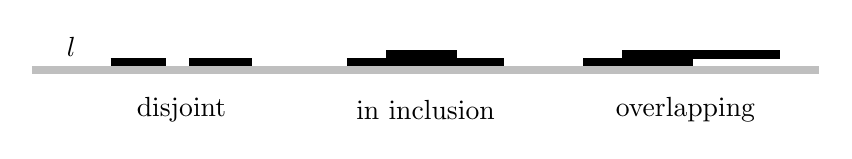
\begin{tikzpicture}
			%% Lines
			\draw[line width = 3, color=lightgray] (0,0) -- (10,0);
			% Disjoint
			\draw[line width = 3, color=black] (1,.10) -- (1.7,.10);
			\draw[line width = 3, color=black] (2,.10) -- (2.8,.10);
			% In inclusion
			\draw[line width = 3, color=black] (4,.10) -- (6,.10);
			\draw[line width = 3, color=black] (4.5,.20) -- (5.4,.20);
			% Overlaping
			\draw[line width = 3, color=black] (7,.10) -- (8.4,.10);
			\draw[line width = 3, color=black] (7.5,.20) -- (9.5,.20);
			%% Text boxes
			\node (l) at (.5,.3) {$l$};
			\node (disjoint) at (1.9, -.5) {disjoint};
			\node (incl) at (5, -.5) {in inclusion};
			\node (overlap) at (8.3, -.5) {overlapping};
		\end{tikzpicture}
		\caption{An illustration to the possible relative positions of pairs of intervals.}
	\end{figure}
	
	\begin{claim}
		If $E_1$ and $E_2$ satisfy the mixing condition, $-G_1$ has an interval intersection representation such that for every two vertices $u, v \in V$, $uv \in \overrightarrow{E_2}$ implies $I_u \subseteq I_v$.
	\end{claim}
	
	\begin{proof}[Proof of claim]
		Let us call a violation a pair of endpoints of intervals $I_u$, $I_v$ with $uv \in \overrightarrow{E_2}$ such that $l_u < l_v$ or $r_v < r_u$. Observe that overlapping intervals provide one violation, while intervals in inclusion provide either $0$ (when $I_u \subseteq I_v$) or $2$ (when $I_v \subseteq I_u$) violations.
		
		Consider a representation $\mathcal{R}$ with the smallest possible number of violations. We will prove that
		this number is zero, i.e., that this $\mathcal{R}$ satisfies the statement of the Claim.
		
		Suppose, for the contrary, that $\mathcal{R}$ has $k > 0$ violations. For every violation, count the number of endpoints of other intervals lying between the two endpoints forming this violation, and let $m$ be the minimum of these counts over all violations. Assume that $\mathcal{R}$ is chosen such that $m$ is minimum possible among all representations with $k$ violations. In the case analysis which follows, we assume that the violation achieving this minimum number of endpoints is formed by the right endpoints of $I_u$ and $I_v$. If it is achieved by their left endpoints, the arguments are similar (and symmetric).
		
		\begin{itemize}[]
			\item \underline{Case $B1$. $m = 0$} Let $r_v < r_u$, with $uv \in \overrightarrow{E_2}$, be a violation such that there are no other endpoints between $r_v$ and $r_u$. Change the representation $\mathcal{R}$ to $\mathcal{R}'$ by changing the interval $I_v$ to $I_v' = [l_v , r_u + \epsilon]$ for a positive $\epsilon$ small enough so that no endpoint of any interval is between $r_u$ and $r_u + \epsilon$ (other intervals remain the same as in $\mathcal{R}$). Then $\mathcal{R}'$ is still an interval intersection representation of $-G_1$, but it has $k - 1 < k$ violations, contradicting the assumption that $k$ was the minimum possible number of violations in an interval representation of $-G_1$.
			
			\item \underline{Case $B2$. $m > 0$} Let $r_v < r_u$, with $uv \in \overrightarrow{E_2}$, be a violation with $m$ endpoints between $r_v$ and $r_u$. Let $P$ be the leftmost of these endpoints.
			
			\begin{itemize}[]
				\item \underline{Subcase $B2\alpha$. $P$ is the right endpoint of an interval.} Let $w \in V$ be such that $P = r_w$. Change the representation $\mathcal{R}$ to $\mathcal{R}'$ by changing the interval $I_v$ to $I_v' = [l_v , r_w + \epsilon]$ for a positive $\epsilon$ small enough so that no endpoint of any interval is between $r_w$ and $r_w + \epsilon$. Then $\mathcal{R}'$ is still an interval intersection representation of $-G_1$. The number of endpoints between $r_v'$ and $r_u$ is $m - 1 < m$. If $\mathcal{R}'$ had the same number of violations as $\mathcal{R}$, this would contradict the assumption of minimality of $m$. Thus $\mathcal{R}'$ must have more than $k$ violations. The only new violation can be formed by $r_w < r_v'$, which means that $vw \in \overrightarrow{E_2}$. Then the transitivity of $\overrightarrow{E_2}$ implies that $uw \in \overrightarrow{E_2}$ and $r_w < r_u$ is a violation in $\mathcal{R}$ with $m - 1 < m$ endpoints between $r_w$ and $r_u$, contradicting the assumption on minimality of $m$.
				
				\item \underline{Subcase $B2\beta$. $P$ is the left endpoint of an interval.} Let $w \in V$ be such that $P = l_w$. Then $I_v \cap I_w = \emptyset$ and hence $vw \in E_1$. The mixing property applied to $u, v, w$ then implies $uw \in E_1$, which is impossible since $P \in I_u \cap I_w \neq \emptyset$.
			\end{itemize}
		\end{itemize}
		
		Thus both Cases $B2$ and $B1$ lead to contradictions, and hence $k = 0$ and $\mathcal{R}$ satisfies the property described in the Claim.
	\end{proof}
	
	Assume we are having an interval intersection representation $\mathcal{R}$ guaranteed by the Claim. It follows that $E_2 \subseteq \mathcal{R}_\text{inclusion}$, and hence $\mathcal{R}_\text{overlap} \subseteq E$. In the first step, define, for every vertex $u \in V$, the interval filament $f_u$ as the half-circle with diameter $I_u$. At this point we observe the following
	
	\begin{enumerate}
		\item if $I_u$ and $I_v$ are disjoint, so are also $f_u$ and $f_v$, which corresponds to the fact that $uv \in E_1$ and thus $uv \notin E$;
		\item if $I_u$ and $I_v$ are overlapping, $f_u$ and $f_v$ cross each other, which corresponds to the fact that $uv \in E$ which is observed above; however
		\item if $I_u$ and $I_v$ are in inclusion, say $I_u \subseteq I_v$, then either $uv \in E_2$ (and thus $uv \in \overrightarrow{E_2}$) or $uv \in E$, but $f_u \cap f_v = \emptyset$ in both cases.
	\end{enumerate}
	
	We will now modify some of the filaments in order to make filaments of case 3 intersect if the corresponding vertices are adjacent in $G$. For every pair of vertices $u, v \in V$ such that $I_u \subseteq I_v$ and $uv \in E$, choose a line $l_u$ perpendicular to the base line $l$ and crossing it in an interior point of $I_u$. Then pull the filament $f_u$ up along $l_u$ to make it cross $f_v$ (cf. an illustrative Fig. \ref{left}). To avoid creating undesired intersections with other filaments, we must modify also those filaments which cross the line $l_u$ between its crossings with $f_u$ and $f_v$. Imagine this as a dynamic process, as if $f_u$ would slowly grow a spike upward and this spike would be pushing every filament $f_w$ in front of it, if $w$ is such that $uw \notin E$. Moreover, if there were another filament $f_z$ above $f_w$ such that $wz \notin E$, $f_z$ would be pushed by $f_w$ etc. See Fig. \ref{right}. We claim that in this way no undesired intersections arise. Such could be only between one of the pushed filaments, say $f_y$, and the filament $f_v$. If $f_y$ is pushed, there is a sequence of vertices $u_0 = u, u_1 , \dots , u_t = y$ such that $f_{u_{i-1}}$ pushes $f_{u_{i}}$ for $i = 1, 2, \dots , t$, i.e., $u_{i-1} u_i \notin E$	and $I_{u_{i-1}} \subseteq I_{u_{i}}$, hence $u_{i-1} u_i \in \overrightarrow{E_2}$. Transitivity of $\overrightarrow{E_2}$ then implies $uy \in \overrightarrow{E_2}$. Similarly, if $f_y$ should not cross $f_v$, i.e., $yv \notin E$, we would have $yv \in \overrightarrow{E_2}$. But that would imply $uv \in \overrightarrow{E_2}$ contradicting the assumption that $uv \in E$.
	
	\begin{figure}[!ht]\centering
		\begin{subfigure}{0.45\textwidth}\centering
			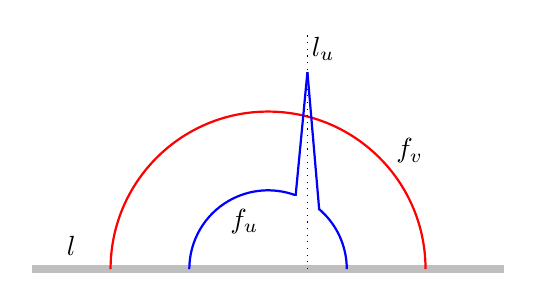
\begin{tikzpicture}
				%% Lines
				\draw[line width = 3, color=lightgray] (0,0) -- (6,0);
				\draw[color=Red, thick] (1,0) arc (180:0:2);
				\draw[color=Blue, thick] (2,0) arc(180:70:1);
				\draw[color=Blue, thick] (4,0) arc(-180:-130:-1);
				\draw[dotted] (3.5, 0) -- (3.5, 3);
				\draw[color=Blue, thick] (3.35,0.93) -- (3.5, 2.5);
				\draw[color=Blue, thick] (3.65,0.75) -- (3.5, 2.5);
				%% Text boxes
				\node (l) at (.5,.3) {$l$};
				\node (lu) at (3.7,2.8) {$l_u$};
				\node (fv) at (4.8,1.5) {$f_v$};
				\node (fu) at (2.7,.6) {$f_u$};
			\end{tikzpicture}
			\caption{Crossing filaments.}
			\label{left}
		\end{subfigure}
		\begin{subfigure}{0.45\textwidth}\centering
			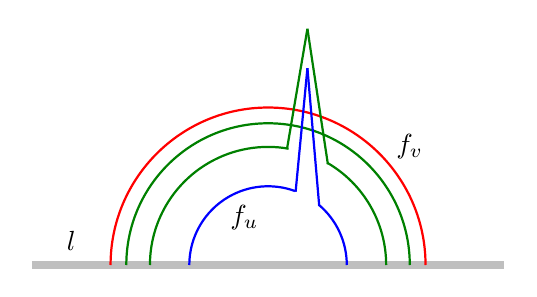
\begin{tikzpicture}
				%% Lines
				\draw[line width = 3, color=lightgray] (0,0) -- (6,0);
				\draw[color=Red, thick] (1,0) arc (180:0:2);
				
				\draw[color=Green, thick] (1.2,0) arc (180:0:1.8);
				
				\draw[color=Blue, thick] (2,0) arc(180:70:1);
				\draw[color=Blue, thick] (4,0) arc(-180:-130:-1);
				\draw[color=Blue, thick] (3.35,0.93) -- (3.5, 2.5);
				\draw[color=Blue, thick] (3.65,0.75) -- (3.5, 2.5);
				
				\draw[color=Green, thick] (1.5,0) arc(180:80:1.5);
				\draw[color=Green, thick] (4.5,0) arc(-180:-120:-1.5);
				\draw[color=Green, thick] (3.24,1.47) -- (3.5, 3);
				\draw[color=Green, thick] (3.76,1.28) -- (3.5, 3);
				%% Text boxes
				\node (l) at (.5,.3) {$l$};
				\node (fv) at (4.8,1.5) {$f_v$};
				\node (fu) at (2.7,.6) {$f_u$};
			\end{tikzpicture}
			\caption{Pushing outwards.}
			\label{right}
		\end{subfigure}
		\caption{Final modification of interval-filaments in the representation.}
	\end{figure}
\end{proof}